\documentclass[11pt]{report}
\usepackage[spanish]{babel}
\usepackage[utf8]{inputenc}
\usepackage{graphicx}
\usepackage{geometry}
\usepackage{fancyhdr}
\usepackage{amsmath}
\usepackage{helvet}
\usepackage{titlesec}
\usepackage{setspace}
\usepackage{tocloft}
\usepackage{hyperref}
\usepackage{csquotes}
\usepackage{placeins}

\usepackage[style=numeric,sorting=none]{biblatex}
\addbibresource{referencias.bib} 

\onehalfspacing
\renewcommand{\familydefault}{\sfdefault}

\geometry{
  letterpaper,
  left=3cm,
  right=2cm,
  top=2.5cm,
  bottom=2cm,
}

\addto\captionsspanish{
  \renewcommand{\contentsname}{Índice}
}
\renewcommand{\cftchapdotsep}{\cftdotsep}  % Para capítulos
\renewcommand{\cftsecdotsep}{\cftdotsep}   % Para secciones
\renewcommand{\cftsubsecdotsep}{\cftdotsep} % Para subsecciones

\titleformat{\chapter}[display]
  {\normalfont\Large\bfseries}
  {\chaptername\ \thechapter}
  {10pt}
  {\huge}
\titlespacing*{\chapter}{0pt}{-20pt}{20pt}  % Ajusta el espaciado aquí

\begin{document}

% Title page
\begin{titlepage}
	\begin{center}
		
\includegraphics[width=0.4\textwidth]{imagenes/logo_ubb.png}\\
		\normalsize FACULTAD DE INGENIERÍA\\
		DEPTO. INGENIERÍA ELÉCTRICA Y ELECTRÓNICA\\[2cm]

		\LARGE \textbf{``Implementación de un Controlador FOC para Motores Brushless con Encoder Utilizando STM32''}\\[6cm]

		\normalsize AUTOR:\\
		RODRIGO FUENTES PEDREROS\\
		\href{https://www.youtube.com/watch?v=dQw4w9WgXcQ}{\phantom{ASDF}}\\[2cm]

		SEMINARIO PARA OPTAR AL TÍTULO DE\\
		INGENIERO DE EJECUCIÓN EN ELECTRÓNICA\\[1cm]

		CONCEPCIÓN – CHILE\\
		AÑO 2024\\
	\end{center}
\end{titlepage}

% Back title page
\begin{titlepage}
	\begin{center}
		
\includegraphics[width=0.4\textwidth]{imagenes/logo_ubb.png}\\
		\normalsize FACULTAD DE INGENIERÍA\\
		DEPTO. INGENIERÍA ELÉCTRICA Y ELECTRÓNICA\\[2cm]

		\LARGE \textbf{``Implementación de un Controlador FOC para Motores Brushless con Encoder Utilizando STM32''}\\[5cm]

		\normalsize AUTOR\\
		RODRIGO FUENTES PEDREROS\\[3cm]

		\large PROFESOR GUÍA:\\
		\large ANGEL ERNESTO RUBIO\\[1cm]
		\large PROFESORES GUÍA ADJUNTO:\\
		\large PEDRO MELIN COLINA
	\end{center}
\end{titlepage}

\normalsize
\pagenumbering{arabic}
\setcounter{page}{3}

\newpage
\tableofcontents

%\newpage
%\listoffigures

%\newpage
%\listoftables


\newpage
\chapter*{Objetivos}
\addcontentsline{toc}{chapter}{Objetivos}
\section*{Objetivo General}
Implementar un controlador de tipo FOC (Control de Campo Orientado) para motores brushless con encoder, utilizando un microcontrolador STM32, que sirva de base para un driver especializado en la robótica competitiva.

\section*{Objetivos Especificos}
\begin{itemize}
	\item Estudiar los principios del Control de Campo Orientado (FOC) y la modulación de espacio vectorial (SVM) para aplicarlos en el diseño del controlador.
	\item Diseñar el hardware para el controlador FOC, con los componentes mínimos necesarios para validar el funcionamiento.
	\item Configurar y programar el microcontrolador para el algoritmo FOC, utilizando las librerías HAL de STM32
	\item Validar el funcionamiento del controlador y proponer posibles mejoras para su aplicación en robótica competitiva.
\end{itemize}

\newpage
\chapter*{Resumen}
\addcontentsline{toc}{chapter}{Resumen}

\newpage
\chapter*{Introducción}
\addcontentsline{toc}{chapter}{Introducción}

\newpage
\chapter{Estado del Arte}

\section{Control Trapezoidal}
El control trapezoidal, también llamado control de 6 pasos, es sin duda alguna el control más sencillo en términos de complejidad de algoritmo y requerimientos de hardware para el control de motores BLDC.

Este control se basa en seguir una secuencia de 6 pasos. En cada paso de la secuencia se polariza solo uno de los devanados del estator. Es decir, se deja una fase polarizada en positivo, una fase polarizada en negativo y otra fase apagada o en alta impedancia. Esta distribución es la que da origen a los 6 pasos. Cada paso se mantiene por 60 grados de giro y cada fase se mantiene polarizada por 120 grados \cite{fisher2014high}.

Para realizar el cambio de fase, lo más común es el uso de las señales BEMF (Back Electromotive Force o fuerza electromotriz de retorno, por sus siglas en inglés). A esta forma de control trapezoidal se le denomina sensorless o sin sensor. Las señales de BEMF son relativamente sencillas de obtener utilizando una serie de resistencias en estrella para obtener un neutro virtual del bobinado y comparadores de voltaje para la detección del pulso en cada fase \cite{shao2003direct}. La desventaja es que estos pulsos a bajas velocidades son demasiado tenues para ser detectados, por lo que el motor debe realizar un arranque en lazo abierto para llegar a la velocidad mínima necesaria para tener pulsos de BEMF detectables de forma estable y desde ahí poder hacer el control en lazo cerrado, dando como resultado que estos motores tengan un casi nulo torque para el arranque, además de tiempos de arranque bastante altos \cite{Gualtieri2018}.

Como solución a esto, se puede agregar el uso de sensores Hall ubicados estratégicamente frente a los imanes del rotor, con el fin de poder identificar en qué paso de la secuencia se encuentra el rotor. A esta configuración se le denomina sensored o con sensor, aunque es posible volver al uso de las señales BEMF después de cierta velocidad, ya que estas señales sufren menos latencia a alta velocidad que los sensores Hall.

De forma opcional, este control puede tener medición de corriente de la fuente de alimentación. Aunque esta medición solo se usa con fines de protección contra sobrecorriente y no tiene ningún efecto sobre el control de lazo cerrado estando dentro del límite establecido.

La mayor desventaja del control trapezoidal es su alto rizado en el torque del motor, lo que da como resultado un motor con baja eficiencia y precisión. Pero su sencillez y bajo coste lo hace ideal para su uso en radio controlados de pequeña escala como drones o autos \cite{juanpere_tecnicas}.

\section{Fundamentos del Control FOC}

El control FOC es solo uno de los diversos tecnicas de control para motores bruhsless o BLDC, existen otras tecnicas como el control de 6 pasos,que es mas usado en controladors ESC de drones por su simplecidad tando de algoritmo como de hardware, ya que no requiere de un encoder para el feedback de posicion y velocidad ni tampoco requiere estrictamente una medicion de Corriente, aun que los ESC de media-alta gama incorporan medicion de corriente de bus para proteccion del motor. tambien existe el control directo de torque, que es mas comun su uso en motores de media alta potencia, aun que existen algunos trabajos despecto a su aplicacion de motores bruhsless y BLCD, los cuales resaltan su beneficio en timpos de respuesta y mayor simplecidad de algoritmo, no existen placas comersiales que implemente esta estrategia de control para su aplicacion en robotica.

\subsection{Transformada Clarke}
\begin{figure}[ht]
	\centering
	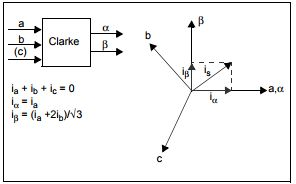
\includegraphics{imagenes/clarke.jpg}
	\caption{Transformada Clarke.}
\end{figure}
\FloatBarrier

\subsection{Transformada Park}
\begin{figure}[ht]
	\centering
	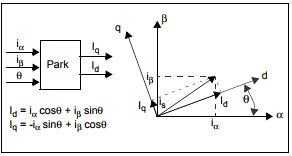
\includegraphics{imagenes/park.jpg}
	\caption{Transformada Park.}
\end{figure}
\FloatBarrier

\subsection{Controladores PI}

\subsection{Transformada Park Inversa}
\begin{figure}[ht]
	\centering
	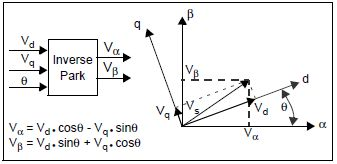
\includegraphics{imagenes/park_inv.jpg}
	\caption{Transformada Park Inversa.}
\end{figure}

\subsection{Modulacion de Espacio Vectorial}

\newpage
\section{Análisis de Proyectos Existentes}
\subsection{Odrive}

\begin{figure}[ht]
	\centering
	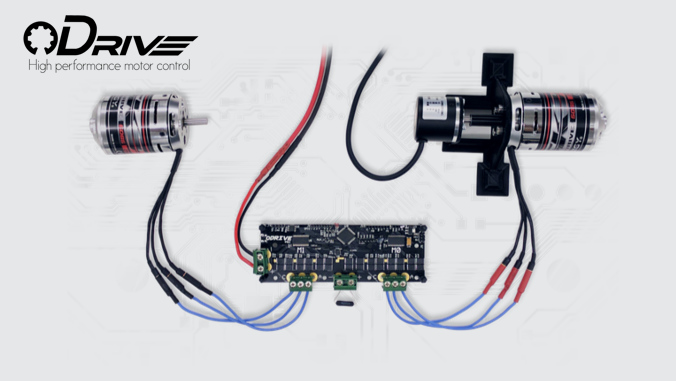
\includegraphics[scale=0.5]{imagenes/odrive_img.jpg}
	\caption{Odrive 3.6}
\end{figure}
\FloatBarrier

Odrive es uno de los controladores FOC comerciales mas populares para su uso en robotica por su gran versatilidad en sus ajsutes y un desempeño exelente para la mayoria de usos. internamente tiene opciones para control de torque, velocidad y posicion.

la version mas popular y generalemtne usada es Odrive 3.6, puede controlar 2 motores de forma simultanea, con hasta 56V y 70A continuos por motor,su codigo es open sourse, aun que solo hasta la vercion 3.5 mantuvo el open hardware, pero actualmente estas verciones estan descontinuadas, ya que el desarrollador esta trabajando en la vercion Odrive PRO.

aun que Odrive tiene un pequeño problema en su forma de operar internamente y es que su bucle se ejecuta a 8000hz, con un PWM de 24.000hz, esto principalemnte limita la electrica maxima que el motor puede controlar a un aproximado de 80.000 ERPM, lo que corresponde a 6 ciclos del bucle por cada giro electronico

\subsection{Vesc project}
\begin{figure}[ht]
	\centering
	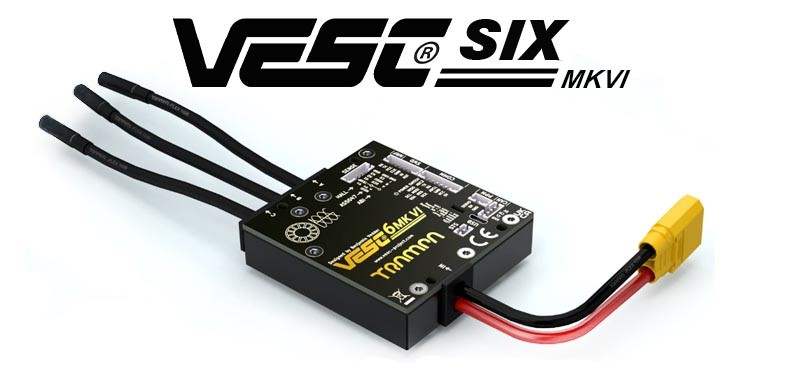
\includegraphics[scale=0.5]{imagenes/Vesc.jpg}
	\caption{Vesc 6}
\end{figure}
\FloatBarrier


\subsection{SimpleFOC}
\begin{figure}[ht]
	\centering
	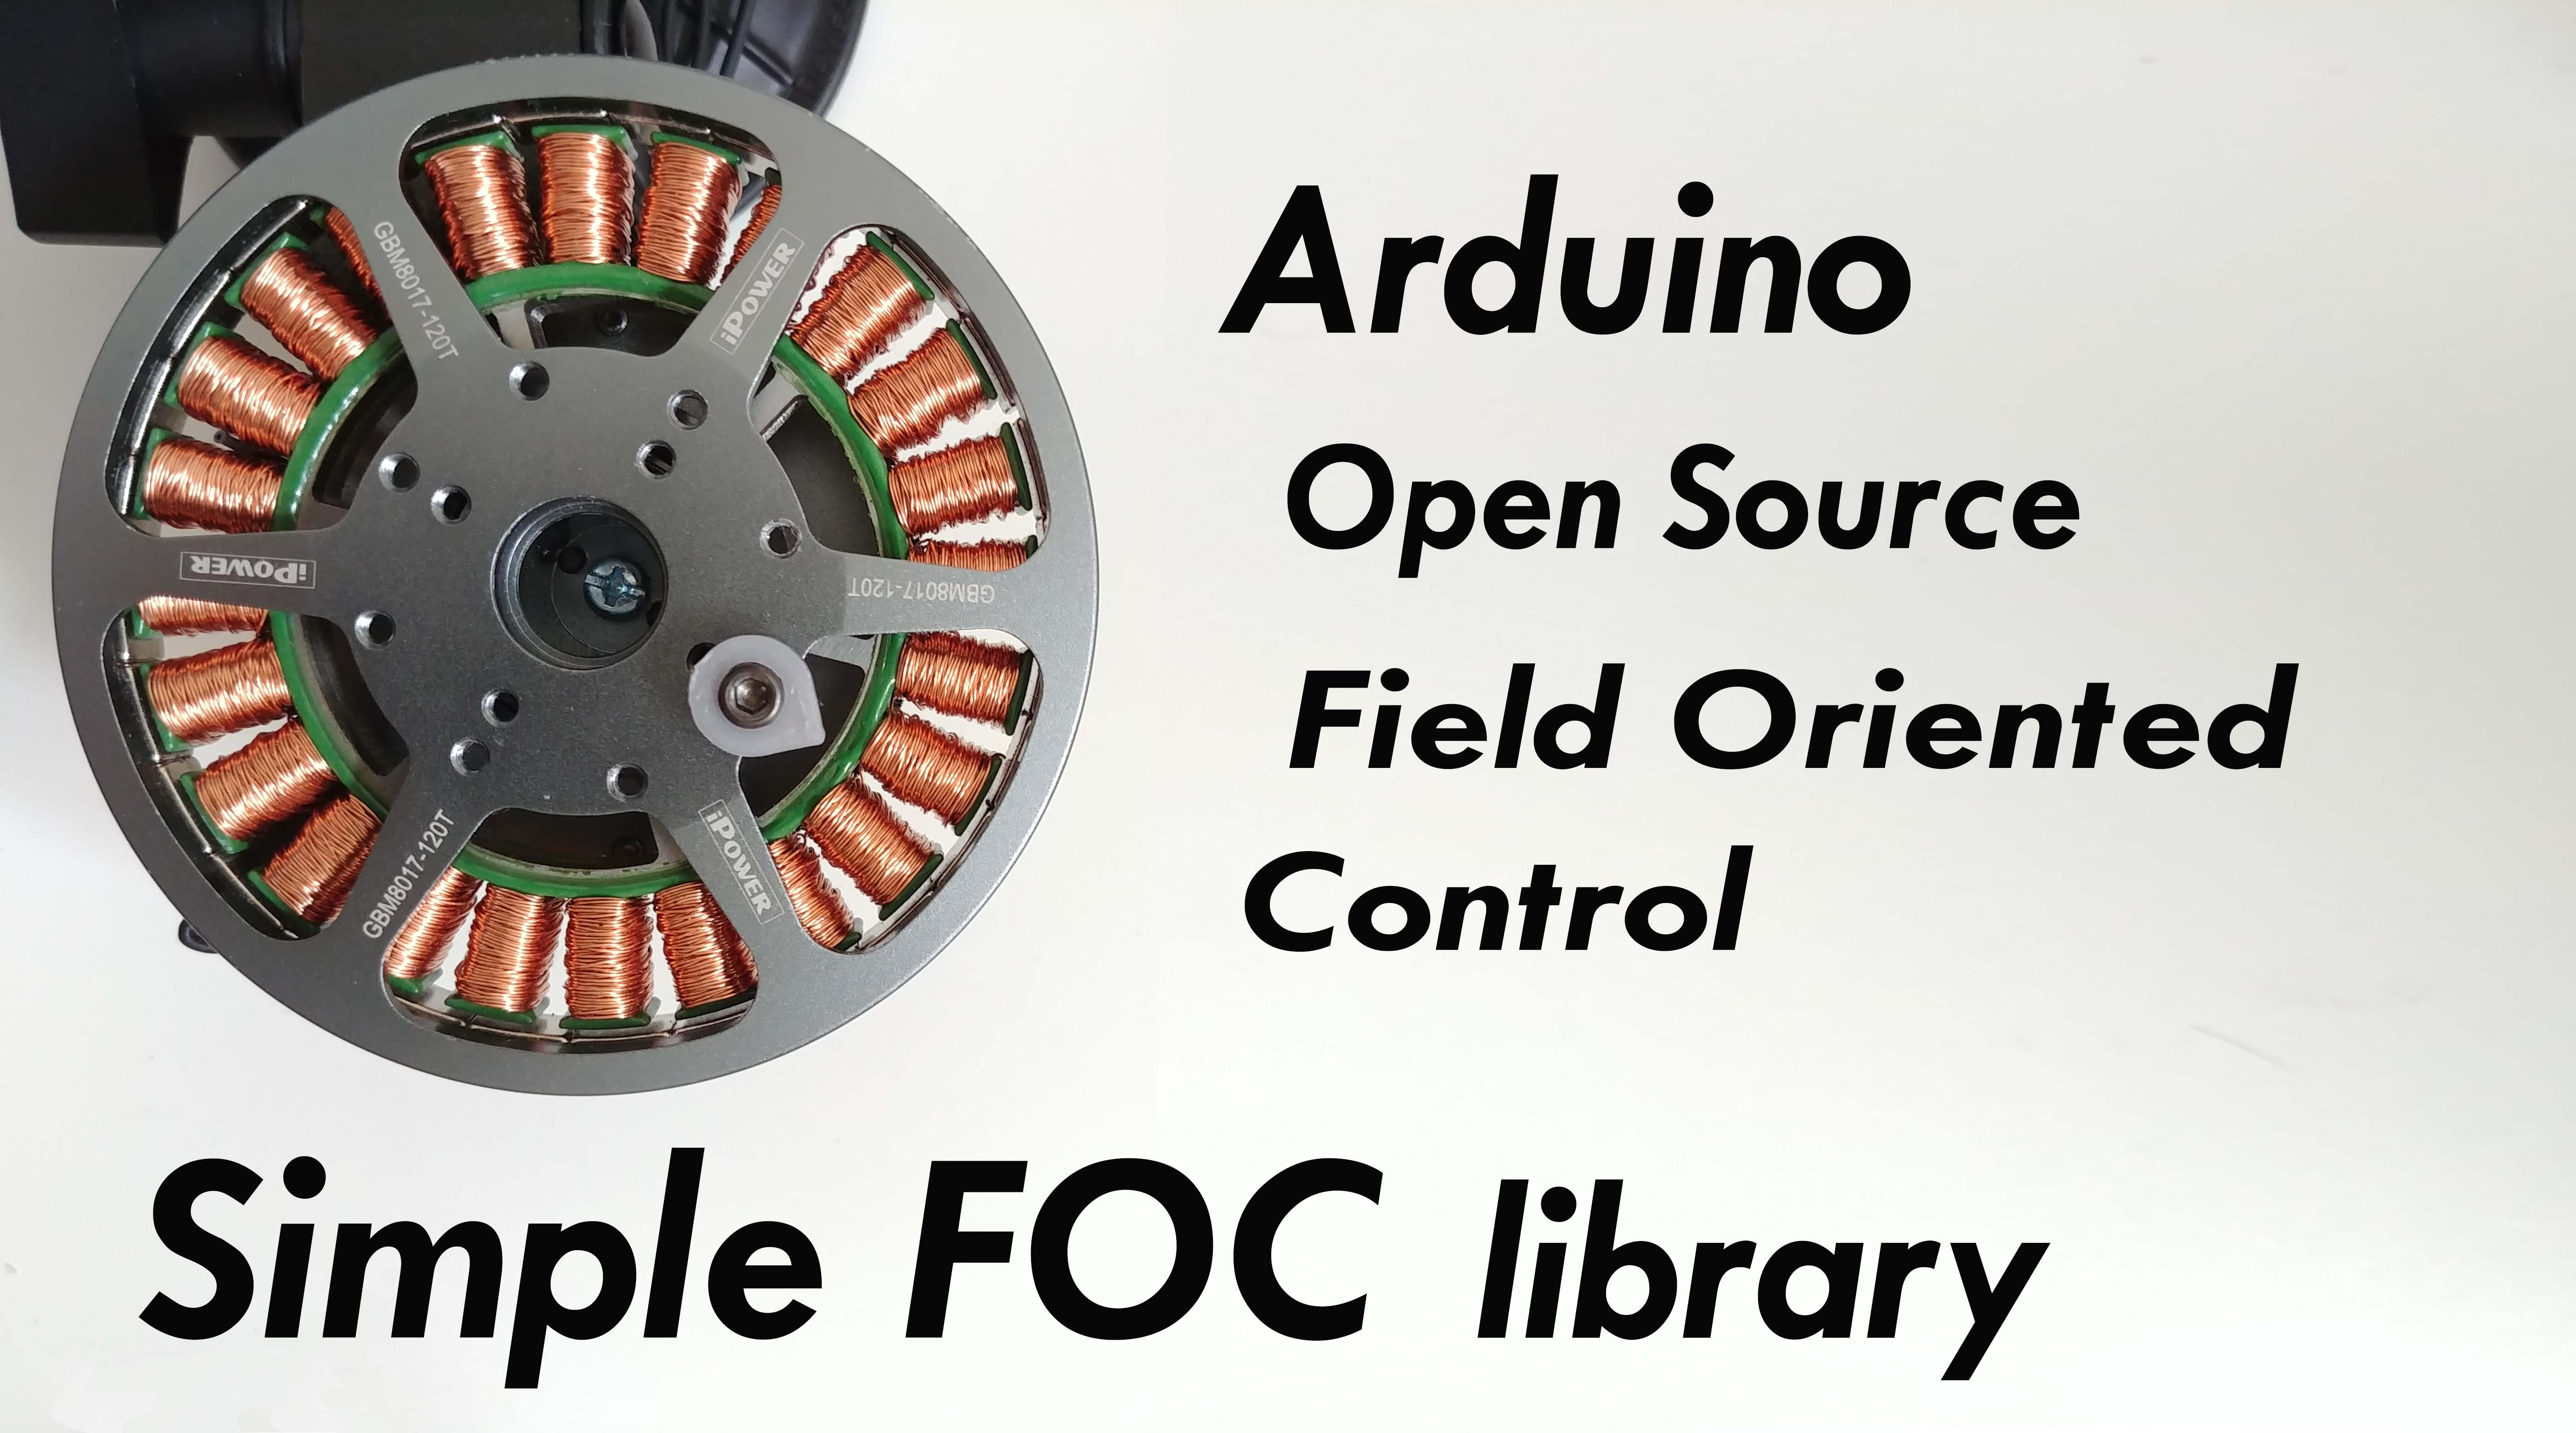
\includegraphics[scale=0.05]{imagenes/simpleFOC.jpeg}
	\caption{SimpleFOC}
\end{figure}
\FloatBarrier

SipleFOC \cite{Skuric_SimpleFOC_A_Field_2022} es una libreria Open Sourse para implementar controladores FOC utilizando arduino IDE o PlatformIO para compilar, este proyecto tiene como foco principa la facilidad de uso, siendo su principal uso en motores de tipo gimbal de baja potencia.

\newpage
\chapter{Diseño de Hardware para el Controlador FOC}
\section{Parametrización del Hardware para el Controlador FOC}
\subsection{Sensores de Corriente}
\subsection{Puente MOSFET}
\section{Implementación del Diseño Electrónico}

\newpage
\chapter{Configuración del STM32 con STM32CubeMX}

\newpage
\chapter{Implementación del Algoritmo de Control FOC}

\newpage
\chapter{Validación y Pruebas de Control FOC}
Este es un documento de ejemplo. Aquí hay una referencia a un libro \cite[p 200]{power_conv_00}.

Este es un documento de ejemplo. Aquí hay una referencia a un libro \cite[p 200]{AN2757_00}.

Este es un documento de ejemplo. Aquí hay una referencia a un libro \cite{odrive_SVM}.

\newpage
\chapter*{Comentarios y Conclusiones}
\addcontentsline{toc}{chapter}{Comentarios y Conclusiones}

\newpage
\addcontentsline{toc}{chapter}{Bibliografía}
\printbibliography

\newpage
\addcontentsline{toc}{chapter}{Anexos}

\chapter*{Anexo A}
\addcontentsline{toc}{section}{Anexo A}

\end{document}
